\chapter{Applying $\mathit{\Phi}$ESTA on real observations}
\label{\thechapter}
\label{ch:Methods}
\addcontentsline{lof}{chapter}{\protect\numberline{\arabic{chapter}} {\nameref{\thechapter}}}

%----------------------------------------------------------------------------------------

\rule{\textwidth}{1.6pt}
\minitoc
\clearpage

%----------------------------------------------------------------------------------------

%{\em CGT: This needs a bit more helpful an introduction. That is WHY the fourier trasform is being explored as
%a way to measure radial velocity. and specifically, so that you can try to tell the difference between bulk line shifts, and line profile deformations.
%I think the folloing does a slightly better job of that.}

\section{HD189733: the Rossiter–McLaughlin effect as jitter}
\label{\thesection}
\label{sec:HD189733}

HD189733 is a well studied binary star system. The main star HD189733~A is known to host a gas giant exoplanet HD189733~b, first detected by transits and subsequently confirmed by Doppler spectroscopy \cite{Bouchy2005ELODIE}. The Rossiter–McLaughlin effect (Fig.~\ref{fig:rm-effect}), is an apparent change in radial velocity produced when the planet passes in front of its parent star, and has been studied in \cite{Cochran2006} and \cite{Triaud2009}. During the eclipse, the planet breaks the observed flux symmetry of the stellar photosphere and produce an asymmetric spectral line profile and apparent radial velocity shift.

%-------------
\begin{figure}[htbp]
\centering
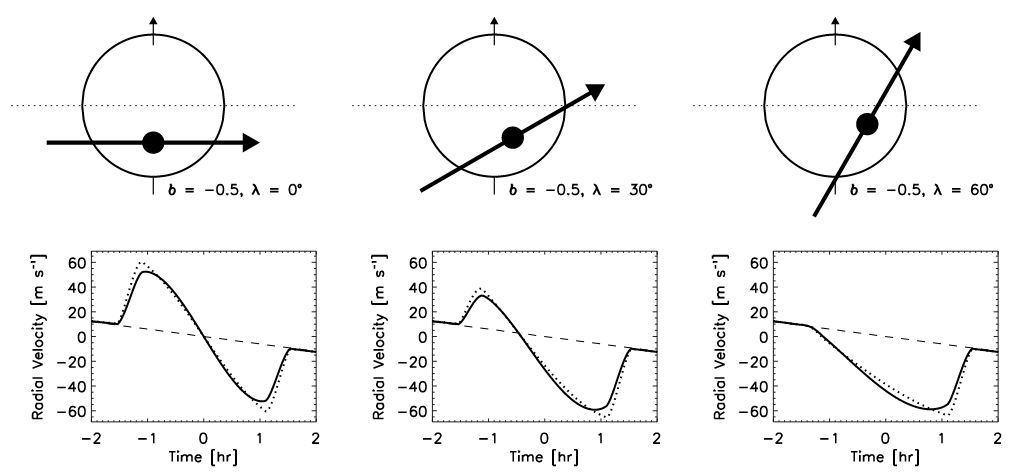
\includegraphics[width = 0.80 \linewidth]
{./Figures/Methods/rmeffect.png}
\caption[The Rossiter–McLaughlin effect]
{The Rossiter–McLaughlin effect (figure taken from \cite{Gaudi2007}) is an apparent radial velocity change of the parent star due to an eclipsing companion (either a star or a planet). This plot shows three different star-planet alignments and the corresponding different forms of Rossiter–McLaughlin curves for each. The solid line is the model including limb darkening, and the dotted line without limb darkening.}
\label{fig:rm-effect}
\end{figure} 
%-------------

We aim to test if jitter estimates generateed by $\mathit{\Phi}$ESTA can account for the apparent radial velocity shift of the Rossiter–McLaughlin effect. We choose this target as a case study for the following reasons: (1) HD189733~b is a confirmed transiting exoplanet, so that we know what to expect from the radial velocity shift during the eclipse. (2) The gas giant exoplanet causes a prominent apparent radial velocity shift as it transits (amplitude up to $\sim 40$~m/s), making it the dominant radial velocity shift (although the star itself exhibits signs of activity \cite{Boisse189733}, \cite{Cauley2017}). (3) The system HD189733 has a visual magnitude of $V\sim7.65$ \cite{SIMBAD189733} (or $G=7.41$ from the Gaia archive), dominated by the primary host star HD189733~A, and therefore a moderate S/N (2000-4000) in the HARPS cross-correlation profile, which is required for $\mathit{\Phi}$ESTA in recovering radial velocities.

There are a few HD189733~b transiting radial velocity segments in the HARPS archive. In particular, we present the one with Julian dates from 2454340.98 to 2454341.11 because it covers both the non-transiting and transiting part of the radial velocity curve and has relatively higher cadence of observing. The cross-correlation of the spectral lines of this segment were constructed by a G2 template by HARPS. We also tested our method in the segment with Julian dates from 2453986.00 to 2453986.17, the cross-correlation profiles of which were constructed by a K5 template, but with about half the observing cadence -- it also returns similar performance on fitting the Rossiter–McLaughlin effect by the $\mathit{\Phi}$ESTA jitter metrics.

Here we briefly recap the procedure for obtaining the ``jitter" model derived by $\mathit{\Phi}$ESTA. $RV_\text{HARPS}$ were obtained from the HARPS spectra headers (consistent with $RV_\text{Gaussian}$ by fitting a Gaussian function to the line profile and $RV_\text{FT}$ derived from the full Fourier phase spectrum); $RV_\text{FT,H}$ and $RV_\text{FT,L}$ were derived from the corresponding part of the Fourier phase spectrum of HARPS cross-correlation line profiles (Fig.~\ref{fig:HD189733} upper left). We could then obtain the raw jitter metrics $\Delta RV_\text{H} = RV_\text{FT,H} - RV_\text{HARPS}$ and $\Delta RV_\text{L} = RV_\text{HARPS} - RV_\text{FT,L}$ (Fig.~\ref{fig:HD189733} lower left). We show only the processes from $\Delta RV_\text{L}$ as the jitter model built from $\Delta RV_\text{H}$ can be obtained in the same procedure and presents similar results. The inclined trend of the radial velocity curve is attributed to the exoplanet (with an orbital period is estimated 2.219 days \cite{Bouchy2005ELODIE}) as well as the companion binary star HD189733~B (with an orbital period $\approx$ 3,200 years \cite{Bakos2006}) -- both orbiting time-scales are long enough compared to the $\sim$ 2 hour planetary transit. Therefore a local approximation can be applied by fitting a linear trend onto the non-transiting part of the radial velocities. This is then removed to leave the residual Rossiter–McLaughlin curve (Fig.~\ref{fig:HD189733} upper right) and treated as ``jitter" and modelled by the raw jitter metric multiplied by a scaling factor. 

%-------------
\begin{figure}[tbp]
\centering
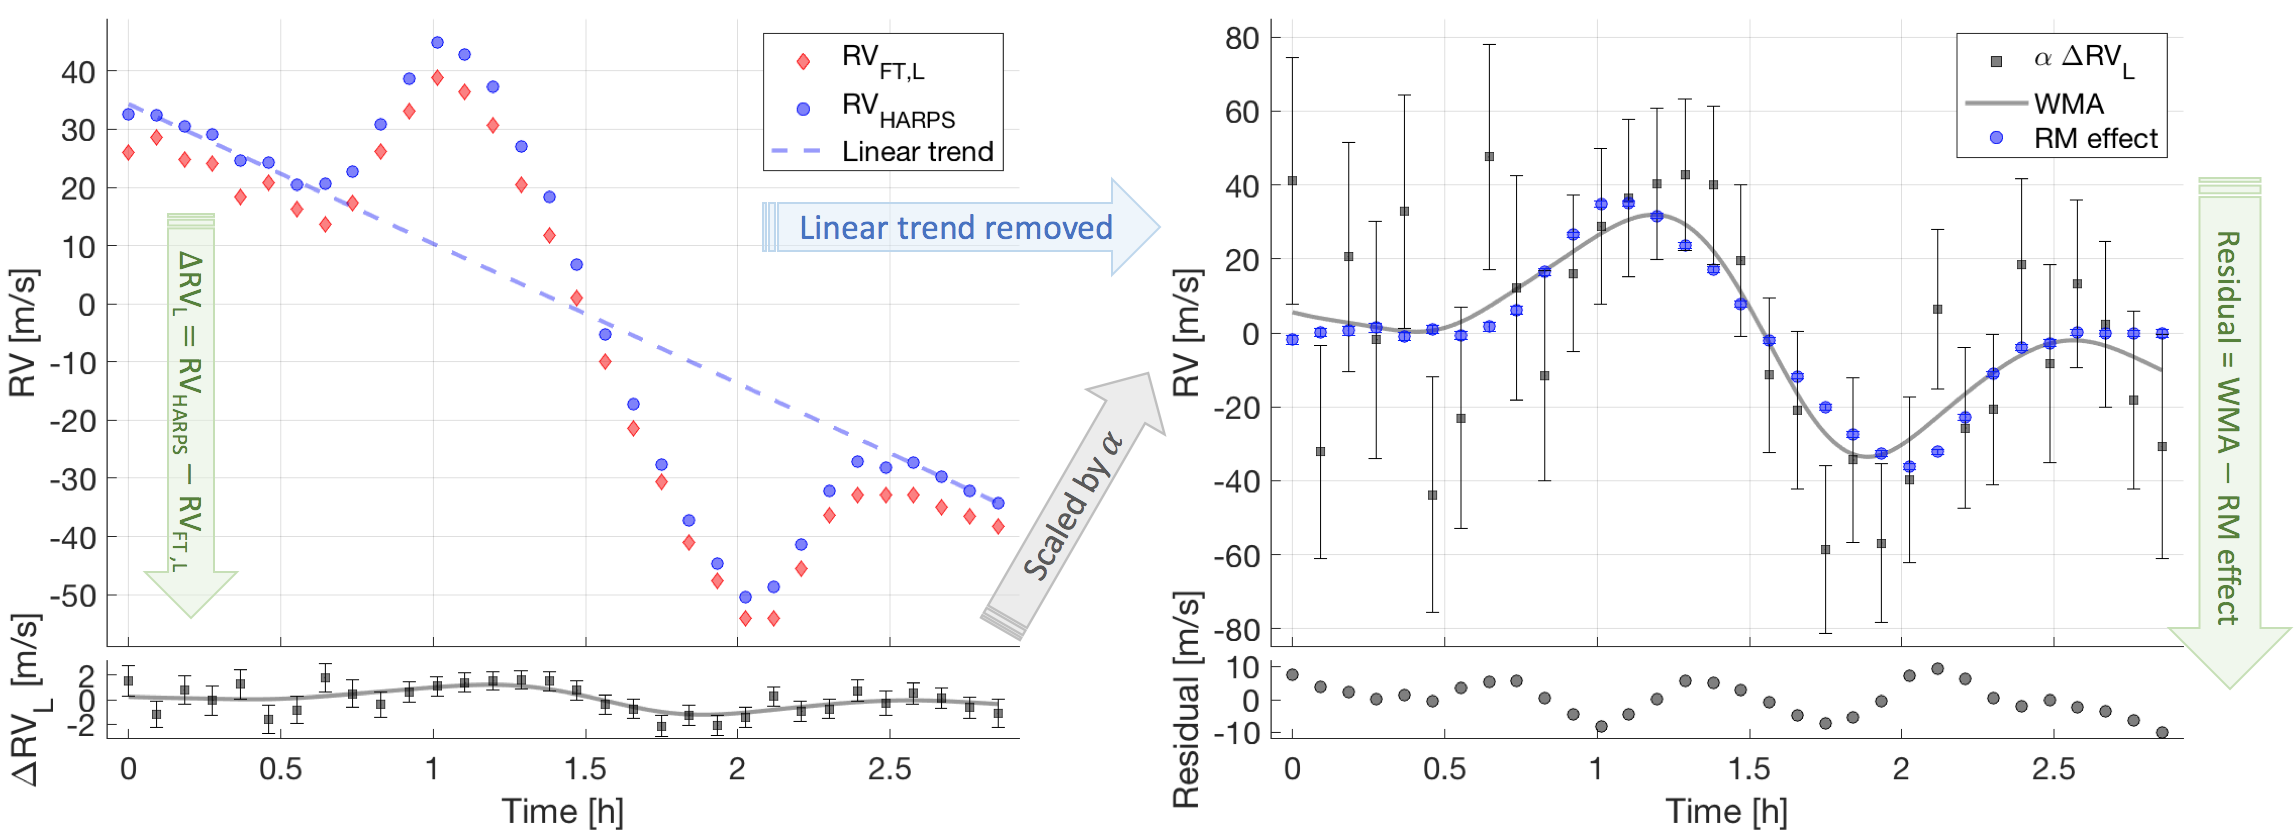
\includegraphics[width = 1.0 \linewidth]
{./Figures/Methods/HD189733.png}
\caption[HD189733: modelling Rossiter–McLaughlin effect as jitter]
		{Flowchart of modelling the Rossiter–McLaughlin effect as jitter using $\mathit{\Phi}$ESTA on HD189733. Note that $RV_\text{FT,L}$ is offset by 5~m/s to avoid visual overlap with $RV_\text{HARPS}$ in the upper left panel. The errorbars related to the radial velocities from $\mathit{\Phi}$ESTA (e.g. $\Delta RV_\text{L}$) are only correct relative to each other (as derived from the photon noise) but not evaluated in the absolute scale.}
\label{fig:HD189733}
\end{figure} 
%-------------

The scaled model is then smoothed using a weighted moving average (WMA) with $\tau~\sim0.2$ hour (twice of the spacing of two consecutive observations). Although required to mitigate against the phase noise sensitivity of $\mathit{\Phi}$ESTA, this does smear the drastic velocity change seen when the planet enters and departs the stellar disk. Fitting a parameterized Rossiter–McLaughlin curve model to the jitter metric instead of smoothing the jitter metric is expected to improve the result. Nevertheless we see that $\mathit{\Phi}$ESTA results in a 75\% removal of the ``jitter" impact of the planetary transit, from $\sim 40$~m/s to $\sim 10$~m/s (Fig.~\ref{fig:HD189733} right). 

%, we still adopt the smoothing approach the way we would normally (intend to) deal with stellar variability induced radial velocities instead, to demonstrate the sufficiently recovered radial velocities as a result of line profile deformation -- a $75\%$ removal of the ``jitter"  

%The effective length of the smoothing kernel should be carefully chosen. In most cases, it can be chosen roughly the same as the spacing between two consecutive exposures. It can be very useful in mitigating the effect of noise (especially for relatively lower S/N data, to which $\mathit{\Phi}$ESTA is sensitive, but in this particular Rossiter–McLaughlin effect during the transit, In the future, an adaptive (e.g. S/N dependent) effective length of the smoothing kernel may be implemented to resolve this problem. 
%
%
%When there's no planet or the planetary radial velocity signal is negligible compared with the size of jitter, $RV_\text{FT,L}$ and $RV_\text{FT,H}$ will be proportional to $RV_\text{jitter}$ (Example: \S\ref{sec:HD189733}).

\section{$\alpha$ Centauri B (HD128621)}
\label{\thesection}

\subsection{Obtain data} 

$\alpha$ Centauri B is a good case study for $\mathit{\Phi}$ESTA due to its brightness (V$\sim$1.33), abundant HARPS observations and the intrinsic stellar activity that brings controversy over whether it hosts an exoplanet. Potentially the (second) closest exoplanet to Earth -- the planet candidate $\alpha$ Centauri Bb was first discovered by \cite{Dumusque_Centauri_B} in 2012, then further investigated by \cite{Hatzes2013} in 2013, and later questioned by \cite{Rajpaul_Alpha_Cen_B} who suggested it was the detection of a ghost signal aliased from the window function. We do not yet seek to address the reality of the planetary candidate, but can study the stellar activity level of $\alpha$ Centauri B, ?? the jitter metrics $\Delta RV_\text{L}$ and $\Delta RV_\text{H}$. In the following, we focus on three segments of the $\alpha$ Centauri B data for activity analysis. Each is roughly one year apart, spans three months and includs over 2000 observations. The specific epochs are -- Epoch 1: 15/02/2009 - 06/05/2009; Epoch 2: 03/23/2010 - 12/06/2010; Epoch 3: 18/02/2011 - 15/05/2011. Among them, Epoch 2 is of particular interest as it has been used to study rotationally modulated stellar activities in K-dwarfs (\cite{Thompson2017MNRAS}, \cite{Wise2018}). 

% \paragraph{Obtain data.}
We downloaded 2617 $\alpha$ Centauri B spectra for Epoch 2 (2010) from the ESO archive, from which we selected the 2529 cross-correlation line profiles that were constructed with a K5 stellar template; the number of observations actually used was then further reduced to 2488 as we took out another 41 observations that presented large radial velocity offsets and visually different cross-correlation line profiles from the rest of the profiles. These removed observations had features at ephemeral time-scales, i.e. their radial velocities stood out from the other observations of the same day in the $RV_\text{HARPS}$, $\Delta RV_\text{H}$ or $\Delta RV_\text{L}$ time-series and they were also classified as outliers in the full width at half maximum (FWHM) indicator, suggesting the presence of stellar flares. Epoch 1 (2009) and 3 (2011) were pre-filtered in a similar manner, resulting in 2220 and 3534 observations used in this analysis.

\subsection{$\mathit{\Phi}$ESTA analysis on $\alpha$ Centauri B's activity}

Fig.~\ref{fig:Alpha_Cen_B} presents the results of $\mathit{\Phi}$ESTA analysis of $\Delta RV_\text{L}$ for these 3 years ($\Delta RV_\text{H}$ is not shown -- it is simply proportional to $\Delta RV_\text{L}$ and works in the same way). We fit the obtained $\Delta RV_\text{L}$ time series with a Gaussian process model described by a quasi-periodic kernel. A Gaussian process model has the advantage of interpreting stochastic processes with a set of flexible forms of functions, constrained by physically motivated covariance kernels. In this case, a quasi-periodic kernel was chosen such that the periodicity can be explained by the rotationally modulated activity and the deviation from periodicity explained by possibly self-evolving disc features (e.g. starspots and plage, differential rotation). Interested readers can refer to the theoretical background on Gaussian processes in a textbook-like literature \cite{Rasmussen2006} or a ``hitchhiker's guide" to Gaussian processes for time-series modelling \cite{Roberts_gaussianprocesses}. For our implementation of the Gaussian process model, we employed the python library \verb|george| delveloped by Foreman-Mackey \cite{Ambikasaran2014}. 

%-------------
\begin{figure}[tbp]
\centering
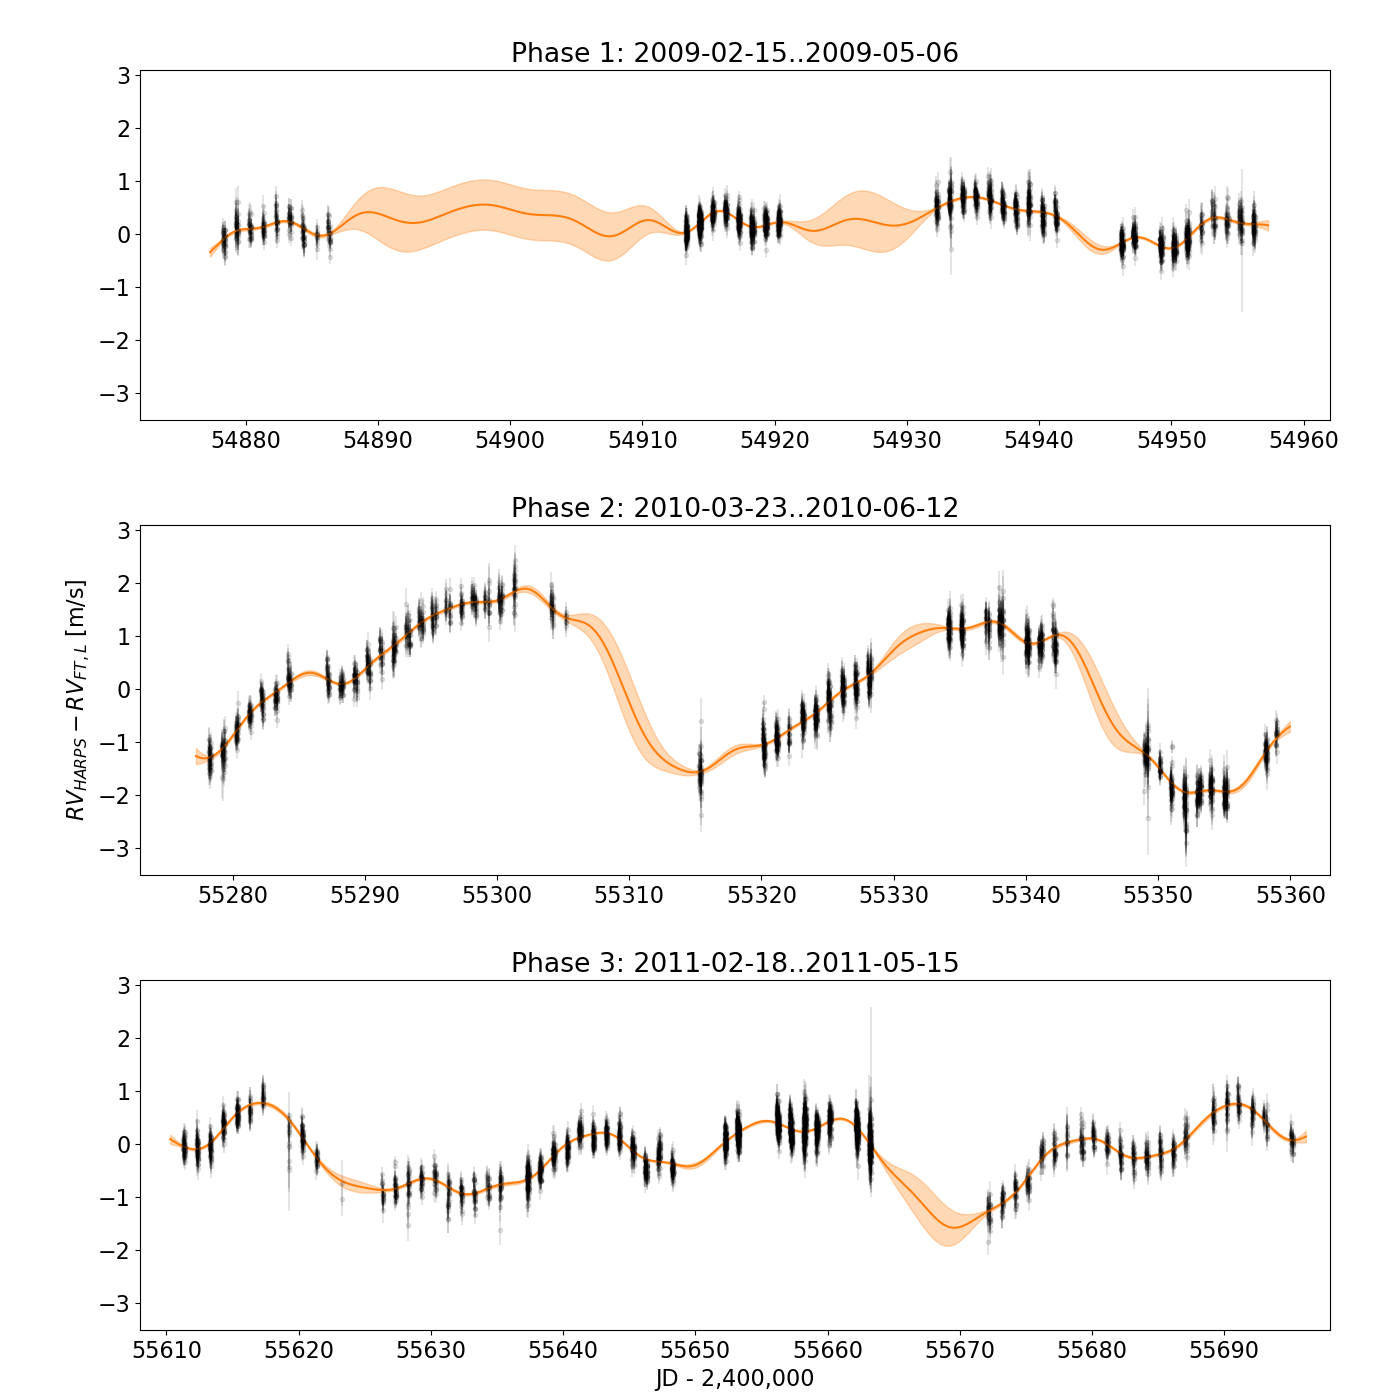
\includegraphics[width = 1.0 \linewidth]
{./Figures/Methods/Alpha_Cen_B.png}
\caption[$\alpha$ Centauri B: stellar activity analysis]
		{Stellar activity analysis of $\alpha$ Centauri B using $\mathit{\Phi}$ESTA. The scaling of the corresponding axes on all subplots are identical. Black dots (with errorbars taken as the photon noise) are the jitter metric $\Delta RV_\text{L}$; the orange solid line is the best fit solution with a quasi-periodic kernel using Gaussian processes and the shaded area is its $1\sigma$ boundary.}
\label{fig:Alpha_Cen_B}
\end{figure} 
%-------------

Fig.~\ref{fig:Alpha_Cen_B} shows that $\alpha$ Centauri B's activity level increased dramatically between 2009 (upper panel) and 2010 (middle panel), and then declined in 2011 (lower panel). In 2010, $\alpha$ Centauri B was dominated by a simple global feature on the stellar surface that appeared with a rotation period of around 40 days, while in 2009 and 2011 the star appears more likely to have been covered by various local features, producing disc inhomogeneity at smaller scales. 

We could obtain the stellar rotation period from our best fit solution with a quasi-periodic kernel in the framework of Gaussian processes. For the three epochs that we studied from 2009 to 2011, we estimate the rotation period to be 37.1, 35.70 and 36.7 days, all consistent with the pre-claimed $36.2\pm1.4$ days \cite{DeWarf2010}. In comparison, \cite{Dumusque_Centauri_B} presented the estimated rotation period to be 39.76, 37.80, 36.71 days respectively for the three years, which was obtained by fitting the radial velocity data by a long-term magnetic cycle model and a stellar rotation described by sine waves accompanied by its harmonics. Note that longer timespans of the three epochs were used by \cite{Dumusque_Centauri_B} to obtain the rotation period. 

A substantial literature has studied the rotationally modulated activity of $\alpha$ Centauri B. The prominent periodicity in 2010 that we present is found to be visually consistent with $\log (R'_\text{HK})$ in original $\alpha$ Centauri Bb discovery paper \cite{Dumusque_Centauri_B}, as well as with the equivalent widths and core flux of activity-sensitive Fe and Mg lines reported in \cite{Thompson2017MNRAS} and \cite{Wise2018}. 

\subsection{Correlations among activity indicators and the radial velocities}

In a more detailed investigation, we present the correlations among a range of existed activity indicators and our jitter metric $\Delta RV_\text{L}$ for the Epoch 2 data of the year 2010 (Fig.~\ref{fig:Correlogram_indicator}). The line core flux (i.e. depth of a line) measurements of Fe 4375.9{\AA} and half-depth range (i.e. width at half-depth flux) measurements of Fe 5250.2{\AA} were shared by \cite{Wise2018} through personal correspondence. The bisector, $\log (R'_\text{HK})$ and the full width at half maximum (FWHM) of the cross-correlation line profiles were taken from the publicized supplementary data file of \cite{Dumusque_Centauri_B}. Since indicators from different sources were binned or selected in their own unique way, we used a moving average to ``interpolate" (and at the same time smooth) all the activity indicators as well as the jitter metric $\Delta RV_\text{L}$ to the same timestamps. 


The two indicators -- bisector and $\Delta RV_\text{L}$, which measure the line deformation in a more direct manner with the unit of a line shift km/s -- are relatively well linearly anti-correlated. There are various parameterizations of a bisector indicator in regards to correlating with an apparent radial velocity shift of a deformed line profile. A commonly used definition would be the difference between the averaged mid point of the top (60-90\%) and bottom (10-40\%) of a line profile, and it has been found to be anti-correlated with the activity-induced radial velocity (\cite{Queloz2001Bis}, \cite{Figueira2013Bis}). The anti-correlation between the bisector indicator and $\Delta RV_\text{L}$ confirms the expected positive correlation between $\Delta RV_\text{L}$ and jitter. 

However, these two indicators do not show a one-to-one correlation with the other indicators studied. This may be because in some circumstances, $\log (R'_\text{HK})$, FWHM, core flux and half-depth range (as well as other indicators that measures flux changes of a line) can become degenerate. For example, while an asymmetric line profile and its mirrored counterpart can be distinguished in $\Delta RV_\text{L}$ and the bisector indicator, they would present the same measurements in $\log (R'_\text{HK})$, FWHM, core flux, half-depth range. As a result, correlating $\Delta RV_\text{L}$ and the bisector indicator with stellar activities would be more reasonable than correlating the $R'_\text{HK}$ activity index with the activity-induced radial velocity, as was used to construct part of the radial velocity model of $\alpha$ Centauri B in \cite{Dumusque_Centauri_B}. In spite of this, the activity indicators of $\log (R'_\text{HK})$, FWHM, core flux and half-depth range show relatively good consistency amongst themselves, especially between $\log (R'_\text{HK})$ and the line core flux. 

%-------------
\begin{figure}[tbp]
\centering
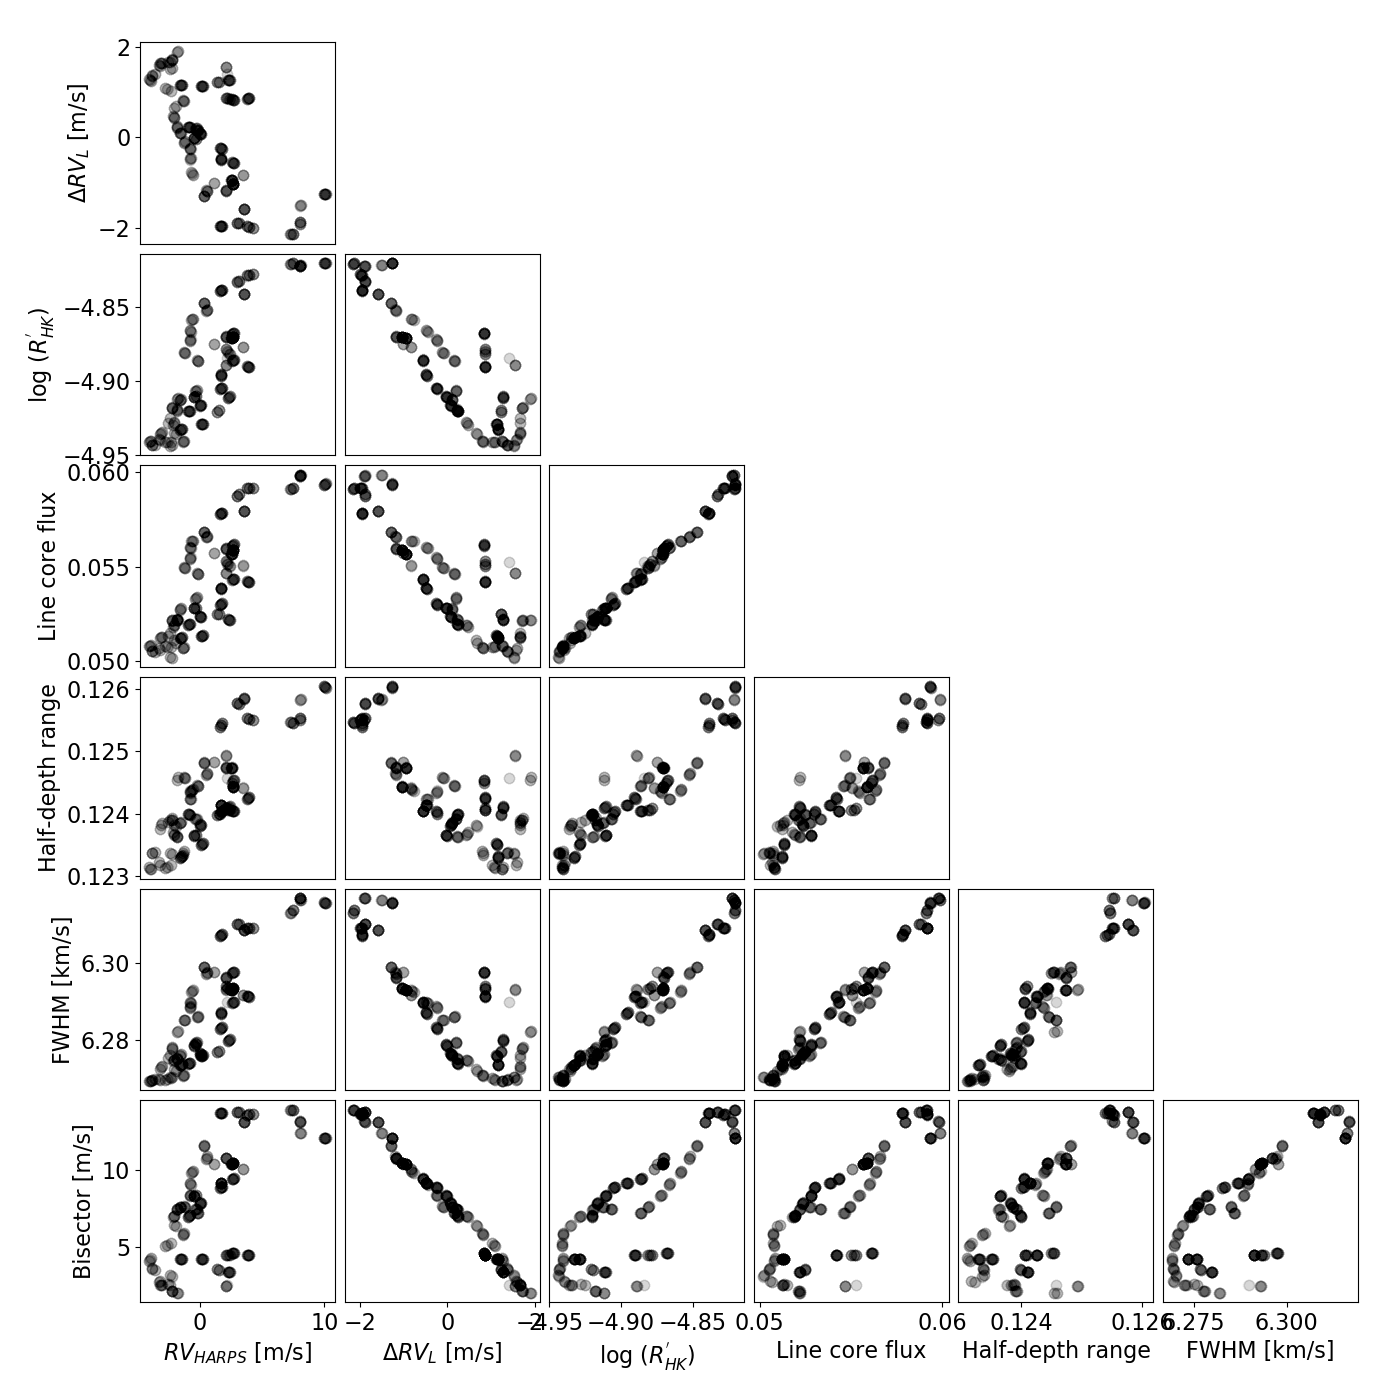
\includegraphics[width = 1.0 \linewidth]
{./Figures/Methods/Correlogram2_indicator_2010.png}
\caption[Correlations among the activity indicators and the jitter metric]
		{Correlations among the 5 activity indicators, the jitter metric $\Delta RV_\text{L}$ and the HARPS radial velocities (minus the binary stellar companion fitted by a second order polinomial) for the Epoch 2 data of $\alpha$ Centauri B in 2010. The line core flux in this plot is a measurement of the line depth of Fe 4375.9 \AA, and the half-depth range is a measurement of the line width at half-depth of Fe 5250.2 \AA, both reproduced from data from \cite{Wise2018}.}
\label{fig:Correlogram_indicator}
\end{figure} 
%-------------

% While our scaled jitter correction $\Delta RV_\text{L}$ in Epoch 2 (2010) does not match with the rotational activity fit of \cite{Dumusque_Centauri_B} and \cite{Hatzes2013}, we do find some shared similarities between our $\Delta RV_\text{L}$ in Epoch 3 (2011) and the corresponding trunk of rotational activity fit presented in \cite{Dumusque_Centauri_B} and \cite{Hatzes2013}, which were obtained using completely different methods from ours. 

In Fig.~\ref{fig:Correlation2010}, we present the correlations among the $\mathit{\Phi}$ESTA and HARPS radial velocities as we demonstrated in \S\ref{sec:Classification} to see if $\mathit{\Phi}$ESTA can provide a quick assessment of whether a system hosts a planet / planets. Unlike the previous simulations, the original HARPS radial velocities include the component of the binary companion $\alpha$ Centauri A. We adopted the same approach and parameters as in \cite{Dumusque_Centauri_B} to remove the binary orbit fitted by a second order polynomial. The results in Fig.~\ref{fig:Correlation2010} are already binary corrected. 

%-------------
\begin{figure}[tbp]
\centering
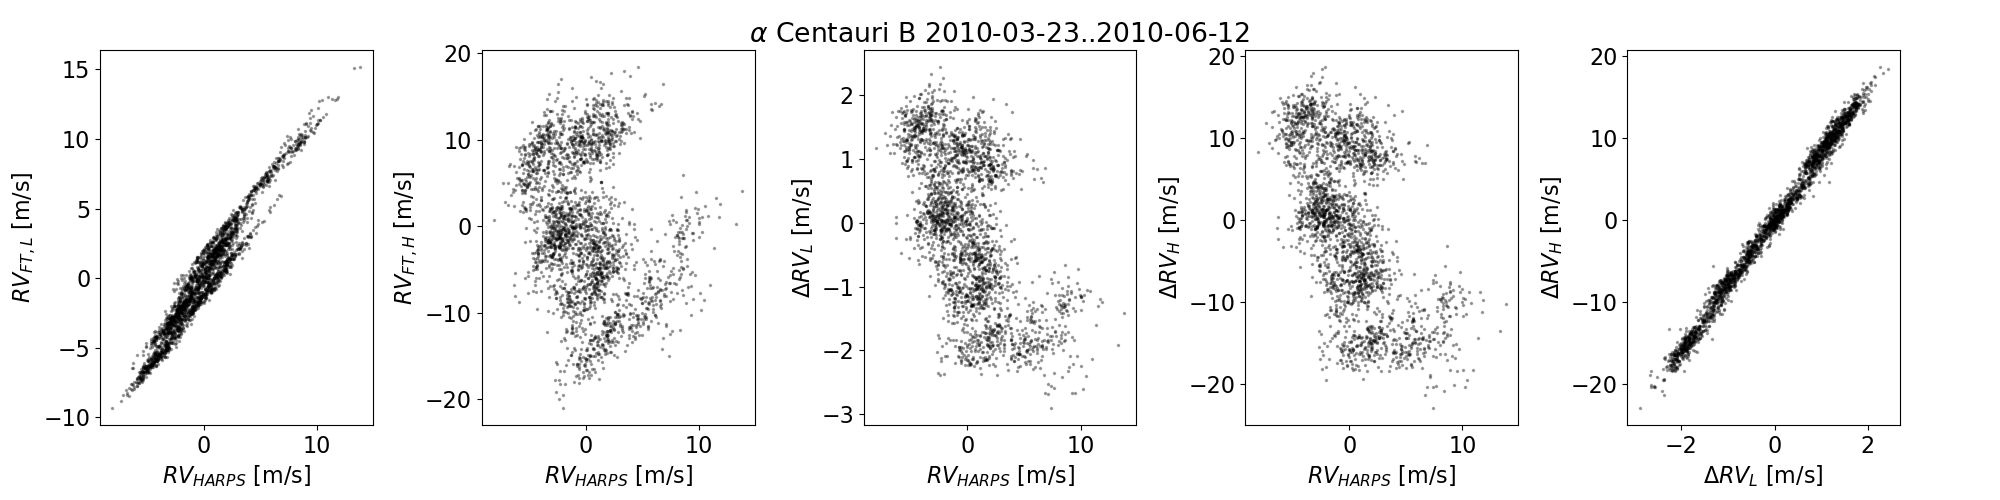
\includegraphics[width = 1.0 \linewidth]
{./Figures/Observations/Correlation2010.png}
\caption[Correlations among the $\mathit{\Phi}$ESTA and HARPS radial velocities]
		{Correlations among the $\mathit{\Phi}$ESTA and HARPS radial velocities.}
\label{fig:Correlation2010}
\end{figure} 
%-------------



\section{$\epsilon$ Eridani (HD22049)}

\section{$\tau$ Ceti (HD10700)}

%HD\,49933 is an F2 main sequence star with an apparent magnitude of $m_V=5.8$ (\cite{Malaroda1975}), 



%%----------------------------------------------------------------------------------------	
\pagebreak
%%----------------------------------------------------------------------------------------	
%----------------------------------------------------------------------------------------
%\clearpage
\section{References}
\label{\thesection}
\vspace{-1.5cm}
\setstretch{1.0}
\bibliographystyle{unsrt}
\bibliography{Bibliography}
\setstretch{1.3}
